\documentclass{beamer}
\usepackage{tikz}
\usepackage{tgheros}       
\usepackage{amsmath, amssymb, amsthm}

\usetheme{BIT}

\usepackage[utf8]{inputenc}

\usepackage{amssymb,amsmath,amsthm}


\usepackage{pgf,tikz}
\usetikzlibrary{arrows}
\usetikzlibrary{shapes,decorations}


% Customize colors for definitionblock

\title{Rings and Ideals}
\author{Filip Zieli\'nski}
\institute[Krakow]{University of the National Education Commission, Krakow.
}
\date{2025}
 
\begin{document}

\begin{frame}
\titlepage
\end{frame}
 
\section{Introduction}

\begin{frame}{Rings}
    \begin{definition}
        A \alert{ring} is a set $R$ equipped with two binary operations denoted (\textbf{$+$}), (\textbf{$\cdot$}) satisfying the following conditions:
        \begin{enumerate}
            \item  The structure $(R, +)$ is an abelian group.
            \item  $\forall x, y, z \in R : (x \cdot y) \cdot z = x \cdot (y \cdot z)$ \hfill \textit{(associativity)} 
            \item  $\forall x, y, z \in R : x \cdot (y + z) = (x \cdot y) + (x \cdot z)$ $\land$ \\
                  $(x + y) \cdot z = (x \cdot z) + (y \cdot z)$ \hfill \textit{(distributivity)} 
        \end{enumerate}
    \end{definition}
    \pause 
    Additionally:
    \begin{enumerate}
        \item \textit{If there exists an identity in a monoid ($R, \cdot$), we say that $R$ is a \alert{ring with identity}}
        \pause 
        \item \textit{If a monoid ($R, \cdot$) is commutative, we say that $R$ is a \alert{commutative ring}.}
    \end{enumerate}
\end{frame}
\begin{frame}{Ring Examples}
    \begin{alertblock}{Remark}
        \begin{enumerate}
            \item Later in this presentation, when we refer to a ring we mean commutative ring with identity.
            \item If binary operations in a ring are implied or natural, we simply write ring $R$ and we treat it like a set. 
        \end{enumerate}
    \end{alertblock}
    \pause
    \begin{example}
    The following structures are Rings:
    \begin{enumerate}
        \item $(\mathbb{Z}, +, \cdot)$ - Ring of integer numbers.   
        \pause 
        \item $\mathbb{R}\left[x_1,\ldots,x_n\right]$ - Ring of polynomials in $n$ variables with real coefficients.
    \end{enumerate}
     
    \end{example}
\end{frame}

\section{Ideals}

\begin{frame}{Ideals}
    \begin{definition}
        Let $R$ be a ring. Let $I \subseteq R$ be any subset of $R$. We say, that $I$ is an \alert{ideal of ring $R$} if following conditions are satisfied:
        \begin{enumerate}
            \item $\forall a,b \in I : a + b \in I$ 
            \item $\forall r \in R \land a \in I : r \cdot a \in I$
        \end{enumerate}
    \end{definition}
    
    \only<2>{\begin{example}
        Let $R = \mathbb{Z}$ be a ring of integers. Then 
        $$ I = \{ a \in R \mid \exists k \in \mathbb{Z} : a = 3\cdot k \} = \{\ldots, -6 , -3, 0, 3, 6, \ldots\}$$
        is an Ideal of $R$. 
    \end{example}
    }
    \only<3>{\begin{example}
        Let $ R= \mathbb{R}[x,y] $ be a ring of real polynomials in two variables, $C = {(x,y) \in \mathbb{R}^2 \mid x-y = 0}$. Then
        $$ I = \{f \in R \mid \forall (x,y) \in C: f(x,y) = 0 \}$$
        is an ideal of $R$.
    \end{example}}
\end{frame}
\begin{frame}{Properties of Ideals}
    \begin{theorem}
        Let $R$ be a ring and let $I,J \subseteq R$ be ideals of $R$. Then $I \cap J$ is an ideal of $R$. 
    \end{theorem}
    \pause
    \begin{proof}
        Let $a,b$ be any elements of $I \cap J$. Then by definition $a \in I \land a \in J \land b \in I \land b \in J$. Since I is an ideal in $R$ and $a,b \in I$ therefore $a + b \in I$. Same can be applied to get $a + b \in J$. Thus $a + b \in I \cap J$. 
        Since $I$ is an ideal of $R$ then for all $r \in R$ $r \cdot a \in I$. Same can be applied to show that for all $r \in R$  it is true that $r \cdot a \in J$. Now we can state the fact that for all $r \in R  r\cdot a \in I \cap J$ which ends the proof.
    \end{proof}
\end{frame}
\section{Geometry of Ideals}
\begin{frame}{Algebraic Sets of an Ideal}
    Let's focus on a case of polynomial ring $R = \mathbb{R}[x,y]$. 
    \begin{definition}
        Let $I$ be an ideal of $R$. We define $V(I)$ to be the intersection of set of roots of every polynomial in $I$:
        $$V(I) = \{ (x,y) \in \mathbb{R}^2 \mid \forall f \in I f(x,y) = 0\}$$
    \end{definition}
    \pause 
    Now, we have defined nice connection between ideals of polynomial ring and sets on a real plane.
\end{frame}
\begin{frame}{Geometry od Ideals }
    \begin{example}
    Let $I = \{ (x-2y)\cdot f \mid f \in R\}$ be an ideal of $R$. Then 
    $$V(I) = \{ (x,y) \in \mathbb{R}^2 \mid x-2y = 0\} = \{(x,\frac{1}{2}x) \in \mathbb{R}^2 | x \in \mathbb{R} \}$$
    \centering
    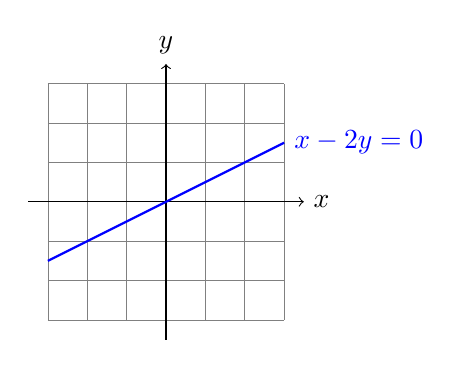
\begin{tikzpicture}[scale = 0.5]
        \draw[very thin, gray] (-3,-3) grid (3,3);
        \draw[->] (-3.5, 0) -- (3.5, 0) node[right] {$x$};
        \draw[->] (0, -3.5) -- (0, 3.5) node[above] {$y$};
        \draw[blue, thick] (-3, -1.5) -- (3, 1.5) node[right] {$x - 2y = 0$};
    \end{tikzpicture}
    \end{example}
\end{frame}
\begin{frame}

\end{frame}

\end{document}